\documentclass[11pt,a4paper]{article}

\usepackage[spanish]{babel}
\usepackage{amsmath,amsfonts, amssymb, mathtools} % Podemos añadir amssymb, amsthm o bm
\usepackage{graphicx, xparse}
\usepackage[top=2cm,bottom=2cm,left=3cm,right=3cm,marginparwidth=1.75cm]{geometry} % Este paquete permite modificar los márgenes del documento
\usepackage[colorlinks=true, allcolors=blue]{hyperref} % Se indica que los hipervínculos van todos en azul
\usepackage{setspace}
\usepackage{xcolor, tcolorbox, booktabs, multirow, colortbl}
\usepackage{cancel} %tachar cosas
\tcbuselibrary{breakable}
\usepackage{hyperref}
\usepackage{titlesec}
\usepackage{array}
\usepackage{tikz}
\usetikzlibrary{positioning,shapes.geometric,fit,backgrounds}
\usepackage{listings, lstautogobble}
\usepackage[T1]{fontenc}
\usepackage[utf8]{inputenc}
\usepackage{fontspec}
\usepackage{makecell}
\usepackage{nicematrix}

\graphicspath{ {images/}}



% Definir lenguaje MiAssembly
\lstdefinelanguage{MiAssembly}{
    keywords={MOV, ADD, SUB, STR, LDR, JMP, CALL, RET, PUSH, POP, MOVL, MOVH, AND, OR, XOR, INC, DEC, NOT, NEG, CMP, JMP, BRC, BRNC, BRO, BRNO, BRZ, BRNZ, BRS, BRNS, JGE, LEA, JNE, JE, MOVSX, SHL, IMUL}, % Instrucciones de ensamblador
    keywordstyle=\color{blue}\bfseries,
    morekeywords=[2]{r0, r1, r2, r3, r4, r5, r6, r7, SP, PC}, % Registros
    keywordstyle=[2]\color{purple}\bfseries,
    morecomment=[l]{;}, % Comentarios con ;
    commentstyle=\color{gray}\itshape,
    morestring=[b]", % Cadenas entre comillas dobles
    stringstyle=\color{verdeSuave},
    sensitive=true, % Diferencia entre mayúsculas y minúsculas
}

% Estilo para Assembly
\lstdefinestyle{assemblyStyle}{
    language=MiAssembly,
    inputencoding=utf8,
    basicstyle=\ttfamily\footnotesize,
    stringstyle=\ttfamily\color{verdeSuave},
    commentstyle=\ttfamily\itshape\color{gray},
    keywordstyle=\color{blue}\bfseries,
    numbers=left,
    numberstyle=\tiny\color{gray},
    xleftmargin=10pt,
    frame=shadowbox,
    breaklines=true,
    extendedchars=true,    
    autogobble=true,
    tabsize=4,
    literate=%
        {á}{{\'a}}1 {é}{{\'e}}1 {í}{{\'i}}1 {ó}{{\'o}}1 {ú}{{\'u}}1
        {Á}{{\'A}}1 {É}{{\'E}}1 {Í}{{\'I}}1 {Ó}{{\'O}}1 {Ú}{{\'U}}1
        {ñ}{{\~n}}1 {Ñ}{{\~N}}1
}
% Estilo para C++
\lstdefinestyle{cppStyle}{
    language=C++,
    inputencoding=utf8,
    basicstyle=\ttfamily\footnotesize,
    stringstyle=\ttfamily\color{verdeSuave},
    commentstyle=\ttfamily\itshape\color{gray},
    keywordstyle=\color{blue}\bfseries,
    numbers=left,
    numberstyle=\tiny\color{gray},
    xleftmargin=10pt,
    frame=trBl,
    frameround=tttt,
    backgroundcolor=\color{gray!20},
    breaklines=true,
    extendedchars=true,    
    autogobble=true,
    tabsize=4,
    literate=%
        {á}{{\'a}}1 {é}{{\'e}}1 {í}{{\'i}}1 {ó}{{\'o}}1 {ú}{{\'u}}1
        {Á}{{\'A}}1 {É}{{\'E}}1 {Í}{{\'I}}1 {Ó}{{\'O}}1 {Ú}{{\'U}}1
        {ñ}{{\~n}}1 {Ñ}{{\~N}}1
}




%Colores
\definecolor{blanco}{HTML}{FFFFFF}
\definecolor{negro}{HTML}{000000}
\definecolor{azulSuave}{HTML}{6ac9d5}
\definecolor{naranjaSuave}{HTML}{d5956a}
\definecolor{verdeSuave}{HTML}{6ad578}
\definecolor{verdeHoja}{HTML}{006400}
\definecolor{naranjaDuro}{HTML}{bd2d0e}



\titleformat{\part}[display]
  {\normalfont\Huge\bfseries} % Estilo del texto
  {}           % Prefijo antes del título de la parte
  {20pt}                      % Separación entre "Parte I" y el título
  {\Huge}                     % Estilo del título de la parte



%Colores
\definecolor{blanco}{HTML}{FFFFFF}
\definecolor{negro}{HTML}{000000}
\definecolor{azulSuave}{HTML}{6ac9d5}
\definecolor{naranjaSuave}{HTML}{d5956a}
\definecolor{verdeSuave}{HTML}{6ad578}
\definecolor{magenta}{HTML}{FF00FF}
\definecolor{dorado}{HTML}{ad8a1f}
\definecolor{amarilloPastel}{RGB}{255, 249, 196} % Amarillo pastel claro
\definecolor{amarilloOscuro}{RGB}{253, 216, 100}  % Amarillo más oscuro
\definecolor{grisSuave}{RGB}{230, 230, 230}      % Gris suave
\definecolor{negro}{RGB}{0, 0, 0}                % Negro puro

\newtcolorbox{dem_box}[1]{
before=\par\smallskip\centering,
colframe=azulSuave!70,
colback=white,
fonttitle=\bfseries,
coltitle=negro,
title=#1,
flushleft title,
width=1\linewidth,
breakable = true
}

\newtcolorbox{ejem_box}[1]{
before=\par\smallskip\centering,
colframe=verdeSuave!70,
colback=white,
fonttitle=\bfseries,
coltitle=negro,
title=#1,
flushleft title,
width=1\linewidth,
breakable = true
}

\newtcolorbox{ej_box}[1]{
before=\par\smallskip\centering,
colframe=naranjaSuave!70,
colback=white,
fonttitle=\bfseries,
coltitle=negro,
title=#1,
flushleft title,
width=1\linewidth,
breakable = true
}

\newtcolorbox{mod_box}[1]{
before=\par\smallskip\centering,
colframe=amarilloOscuro!85,
colback=amarilloPastel!30,
fonttitle=\bfseries,
coltitle=negro,
title=#1,
flushleft title,
width=0.94\textwidth,
breakable = true
}



\setstretch{1.2}
\decimalpoint

% \title{\textbf{BASES DE DATOS: } EJERCICIOS RESUELTOS}
% \author{Diego Díaz Mendaña}
%\date{Fecha}

\begin{document}

\begin{titlepage}
    \begin{center}
        % Logo de la institución
        
\includegraphics[width=0.3\textwidth]{logo_escuela.png} \\[1cm] % Cambiar logo_escuela por el nombre del archivo con el logo
        \vspace{1cm}
        
        \textbf{\LARGE ESCUELA DE INGENIERÍA INFORMÁTICA DE OVIEDO} \\[1.5cm]
        
        \rule{\linewidth}{0.5mm} \\[0.4cm]
        \textbf{\Huge Fundamentos de Computadores Y Redes} \\[0.3cm]
        \rule{\linewidth}{0.5mm} \\[1cm]
        
        {\Large Curso 2024-2025} \\[1.5cm]
        
        \textbf{\LARGE Trabajo Grupal - Fase II} \\[0.8cm]
        
        \text{Díaz Mendaña, Diego - UO301887}\\[0.15cm]
        \text{García Pernas, Pablo - UO300167}\\[0.15cm]
        \text{Gota Ortín, Jorge - UO301023}\\[0.15cm]
        \text{Suárez Fernández, Fernando - UO300028}
        
        \vfill
        
        % Información del alumno
        \begin{flushright}
            \textbf{Grupo de prácticas:} PL.3 - A \\[0.3cm]
            \textbf{Titulación:} PCEO Informática y Matemáticas \\[0.3cm]
        \end{flushright}
        
        \vfill
        
        \today \\[1cm]
    \end{center}
  \end{titlepage}

\newpage
\hypersetup{linkcolor=black}
\tableofcontents
\hypersetup{linkcolor=blue}
\newpage

\section{Introducción}
La presente memoria tiene por objetivo documentar de manera exhaustiva el desarrollo de la Fase II del trabajo práctico correspondiente a la asignatura \textbf{Fundamentos de Computadores y Redes}. El propósito fundamental de esta fase consiste en profundizar en los conceptos generales abordados previamente en los laboratorios de la materia, aplicándolos en un contexto de análisis práctico. \vspace{2ex}

\noindent En particular, la práctica propuesta requiere llevar a cabo el análisis detallado del código fuente de un programa, utilizando para ello las herramientas de depuración que proporciona el entorno de desarrollo \textbf{Visual Studio}. A través de este análisis, se pretende identificar las palabras clave necesarias para la desactivación de una ``bomba binaria''. Como actividad final, se procederá a modificar el código de manera que la bomba no explote independientemente de las entradas proporcionadas por el usuario. \vspace{2ex}

\vspace{3ex}

\section{Desarrollo del análisis de las palabras clave}

El programa objeto de análisis ha sido suministrado por el profesor de la asignatura y se encuentra ubicado en la carpeta denominada \textit{bomba} de este repositorio, concretamente en el archivo ejecutable \texttt{main.exe}. Este ejecutable, diseñado para el sistema operativo Windows, solicita durante su ejecución una serie de entradas por parte del usuario. En caso de que dichas entradas sean correctas, el programa continúa su ejecución sin incidentes, en caso contrario, la ``bomba'' programada explota (la demostración de este comportamiento queda fuera del alcance de la presente memoria). \vspace{2ex}

\noindent El programa en cuestión se encuentra estructurado en cuatro etapas, cuya ejecución secuencial condiciona la desactivación segura de la bomba. En los apartados siguientes, se describirá detalladamente el comportamiento observado en cada una de estas fases.\vspace{2ex}

\noindent Para llevar a cabo el análisis de cada etapa, se han empleado las herramientas de depuración integradas en Visual Studio, tales como el \textbf{depurador}, el \textbf{desensamblador} y el \textbf{analizador de memoria}. Al iniciar la depuración del programa, se realiza el desensamblado inicial del código, obteniendo el siguiente resultado:

\begin{center}
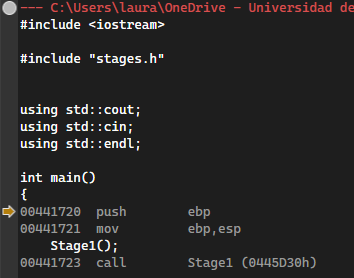
\includegraphics[width=0.5\textwidth]{desarrollo-i.png}
\end{center}

\noindent En este fragmento desensamblado puede observarse que, en la tercera línea de código, mediante la instrucción \texttt{call}, se invoca al procedimiento \texttt{Stage1}. Para analizar el comportamiento de dicho procedimiento, se procede a avanzar la ejecución con dos pulsaciones de \texttt{F10} (para ejecutar las instrucciones línea a línea) y, a continuación, con \texttt{F11} para ingresar dentro del procedimiento y examinar su contenido en profundidad.

\vspace{3ex}


\subsection{Primera etapa}
Una vez que se accede al procedimiento \texttt{Stage1}, se observa el siguiente fragmento de código desensamblado:
\begin{center}
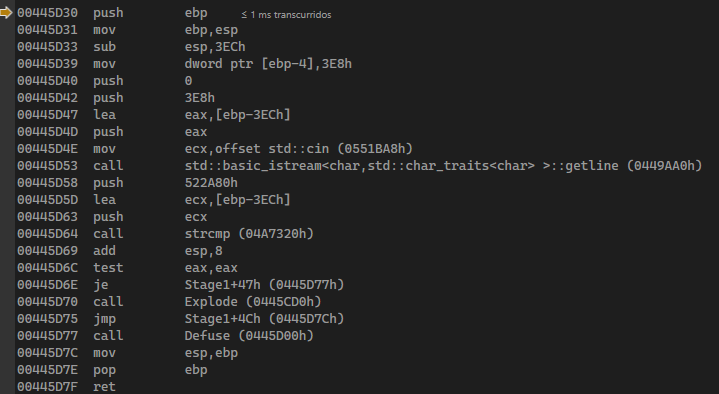
\includegraphics[width=0.95\textwidth]{s1-1.png}
\end{center}

\noindent De forma resumida, puede apreciarse que el procedimiento inicialmente reserva espacio en la pila con el propósito de almacenar una cadena de gran tamaño. Posteriormente, emplea la función \texttt{std::getline} para leer una línea completa de texto ingresada por el usuario a través de \texttt{std::cin}. A continuación, el contenido introducido se compara con una cadena predefinida mediante la función \texttt{strcmp}:

\begin{itemize}
  \item Si la comparación resulta exitosa, el programa invoca el procedimiento \texttt{Defuse}, que desactiva la fase correspondiente.
  \item En caso contrario, se llama a \texttt{Explode}, desencadenando un fallo catastrófico.
\end{itemize}

\noindent En este punto, resulta de gran interés determinar cuál es la cadena correcta que debe ser ingresada para evitar la detonación, preservando así la integridad del programa y, metafóricamente, del ``mundo''.

\vspace{3ex}

\subsubsection{Obtención de la cadena}

\noindent Para identificar la cadena correcta, es crucial examinar la instrucción:

\vspace{1ex}
\begin{lstlisting}[style=assemblyStyle]
  PUSH 522A80h
\end{lstlisting}
\vspace{2ex}

\noindent Dicha instrucción revela la dirección de memoria (\texttt{522A80h}) en la cual se encuentra almacenada la cadena predefinida con la que se realizará la comparación. Por tanto, resulta fundamental acceder al contenido de dicha dirección para obtener la secuencia exacta que debe introducirse. Para ello, se hace uso del analizador de memoria de Visual Studio, introduciendo la dirección mencionada. El resultado del análisis es el siguiente:\vspace{1ex}
\begin{center}
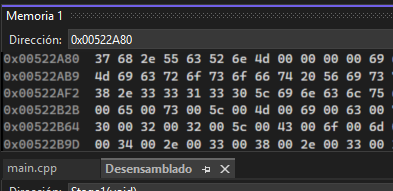
\includegraphics[width=0.7\textwidth]{s1-2.png}
\end{center}
\vspace{2ex}

\noindent En el análisis de memoria se observa que la secuencia de bytes correspondiente es \texttt{37 68 2e 55 63 52 6e 4d 00}. Cabe destacar que en C++ las cadenas de caracteres finalizan con el byte \texttt{00}, indicando el carácter nulo de terminación (\texttt{$\backslash$0}). A partir de la interpretación de estos valores, se concluye que la cadena correcta que debe ser introducida es: \texttt{7h.UcRnM}.\vspace{3ex}

\noindent Una vez introducida dicha cadena durante la ejecución del programa, si se continúa la depuración avanzando con \texttt{F10}, el procedimiento culminará invocando a \texttt{Defuse} y, posteriormente, ejecutará una instrucción \texttt{ret} para regresar al \texttt{main}, mostrando el siguiente código en pantalla:

\begin{center}
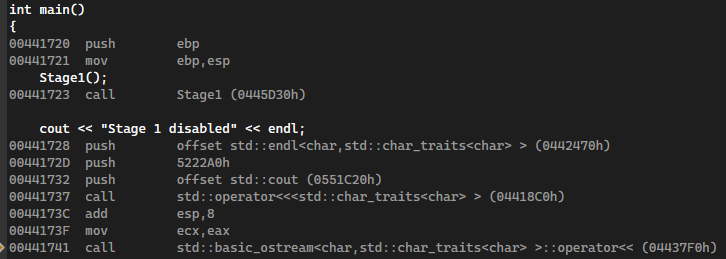
\includegraphics[width=0.95\textwidth]{s1-3.png}
\end{center}

\noindent Asimismo, la consola presentará el siguiente aspecto:
\begin{center}
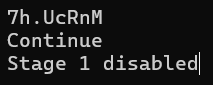
\includegraphics[width=0.4\textwidth]{s1-4.png}
\end{center}
\vspace{3ex}

\subsection{Segunda etapa}

A continuación, en el flujo de ejecución del procedimiento \texttt{main}, puede observarse una invocación a la segunda etapa mediante la instrucción \texttt{call Stage2}. Siguiendo la misma metodología previamente establecida, se accede al procedimiento \texttt{Stage2} utilizando \texttt{F11}, y se procede a desensamblar su contenido, obteniéndose el siguiente resultado:

\begin{center}
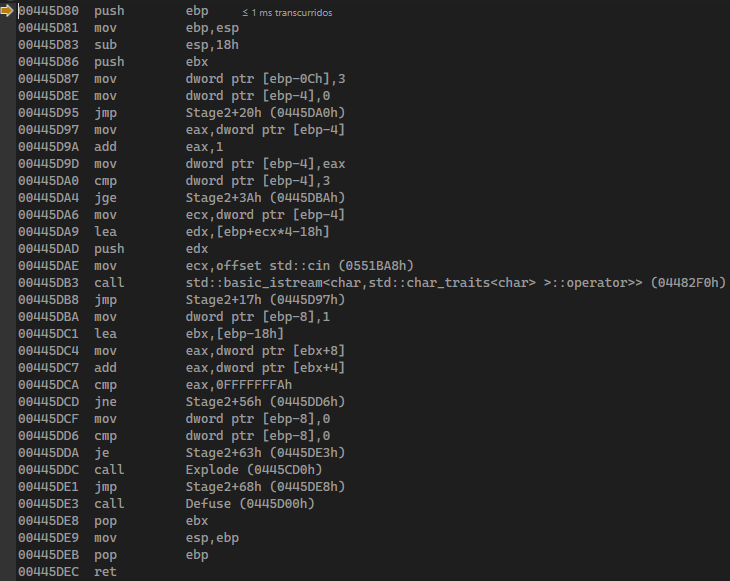
\includegraphics[width=0.95\textwidth]{s2-1.png}
\end{center}

\noindent El código resultante presenta una estructura similar a la observada en la primera etapa: reserva espacio en la pila y configura algunas variables locales necesarias para el control del flujo de ejecución. Posteriormente, se lleva a cabo la siguiente secuencia de operaciones:

\begin{enumerate}
  \item Se establece un bucle que se repite exactamente tres veces, en el cual se solicita al usuario la introducción de un valor numérico a través de \texttt{std::cin}.
  \item Se realizan comprobaciones y operaciones específicas sobre los números ingresados para verificar ciertas condiciones.
  \item Si todas las verificaciones son satisfactorias, se invoca el procedimiento \texttt{Defuse}; en caso contrario, se llama a \texttt{Explode}.
\end{enumerate}

\subsubsection{Condiciones para los valores introducidos}
\noindent Al analizar en detalle la estructura del procedimiento, destacan los siguientes aspectos:
\begin{enumerate}
  \item \textbf{Inicialización de variables:} Se inicializa una variable local con el valor 3 para controlar el número de iteraciones: \vspace{1ex}
  \begin{lstlisting}[style=assemblyStyle]
    00445D0F MOV dword ptr [ebp-0Ch], 3
  \end{lstlisting}
  Seguidamente, se inicializa otra variable local con el valor 0, la cual actuará como contador: \vspace{1ex}
  \begin{lstlisting}[style=assemblyStyle]
    00445D16 MOV dword ptr [ebp-4], 0
  \end{lstlisting}
  \vspace{1ex}

  \item \textbf{Inicio del bucle:} Se efectúa un salto al control del bucle mediante: \vspace{1ex}
  \begin{lstlisting}[style=assemblyStyle]
    00445D1D JMP Stage2+20h (00445D0Ah)
  \end{lstlisting}
  \vspace{1ex}

  \item \textbf{Cuerpo del bucle:} En cada iteración, se incrementa el contador con: \vspace{1ex}
  \begin{lstlisting}[style=assemblyStyle]
    00445D9A MOV eax, 1
    00445D9F ADD dword ptr [ebp-4], eax
  \end{lstlisting}
  \vspace{1ex}

  Una vez que el contador alcanza el valor 3, se abandona el bucle: \vspace{1ex}
  \begin{lstlisting}[style=assemblyStyle]
    00445DA2 CMP dword ptr [ebp-4], 3
    00445DA6 JGE Stage2+3Ah (00445DBAh)
  \end{lstlisting}
  \vspace{1ex}

  Durante las iteraciones, se leen los números ingresados por el usuario: \vspace{1ex}
  \begin{lstlisting}[style=assemblyStyle]
    00445DA8 MOV ecx, dword ptr [ebp-4]
    00445DAB LEA edx, [ebp+ecx*4-18h]
    00445DAF PUSH edx
    00445DB0 MOV ecx, offset std::cin
    00445DB5 CALL std::basic_istream<char>::operator>>
  \end{lstlisting}
  \vspace{1ex}

  Cada número leído se almacena en una dirección diferente dentro de la pila (\texttt{[ebp-18h]}, \texttt{[ebp-14h]} y \texttt{[ebp-10h]}).\vspace{2ex}


  \item \textbf{Comprobaciones:} Finalizada la lectura de los tres números, se procede a verificar que la suma de los dos últimos (\texttt{[ebp-14h]} y \texttt{[ebp-10h]}) sea igual a \(-6\). Si esta condición se cumple, se invoca \texttt{Defuse}; de lo contrario, se llama a \texttt{Explode}: \vspace{1ex}
  \begin{lstlisting}[style=assemblyStyle]
    00445DBA  MOV    dword ptr [ebp-8],1    ; Variable de estado
    00445DC1  LEA    ebx,[ebp-18h]          ; Dirección de los números
    00445DC4  MOV    eax,dword ptr [ebx+8]  ; Carga el tercer número
    00445DC7  ADD    eax,dword ptr [ebx+4]  ; Suma con el segundo número
    00445DCA  CMP    eax,0FFFFFFFAh         ; Compara con -6
    00445DCD  JNE    Stage2+56h (0445DD6h)  ; Si no son iguales, salta
    00445DCF  MOV    dword ptr [ebp-8],0
    00445DD6  CMP    dword ptr [ebp-8],0  
    00445DDA  JE     Stage2+63h (0445DE3h)  
    00445DDC  CALL   Explode (0445CD0h)  
    00445DE1  JMP    Stage2+68h (0445DE8h)  
    00445DE3  CALL   Defuse (0445D00h)
  \end{lstlisting}
  \vspace{1ex}

  \item \textbf{Finalización:} Tras completar la verificación y realizar la llamada pertinente a \texttt{Defuse} o \texttt{Explode}, el procedimiento finaliza y retorna el control al \texttt{main} mediante la instrucción \texttt{ret}.
\end{enumerate}

\noindent Por consiguiente, para superar esta segunda etapa con éxito, el usuario deberá introducir tres valores numéricos de los cuales la suma de los dos últimos sea igual a \(-6\). Tras la ejecución correcta, el resultado en Visual Studio será el siguiente:
\begin{center}
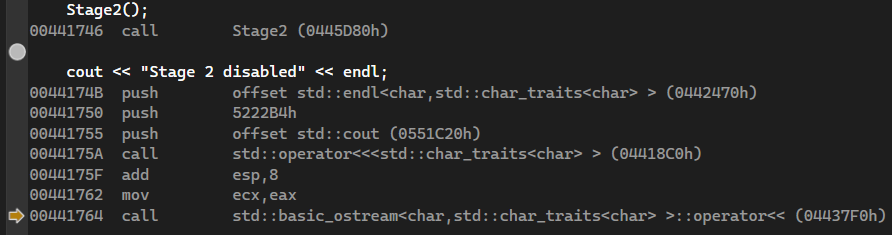
\includegraphics[width=0.9\textwidth]{s2-2.png}
\end{center}

\noindent Y la consola mostrará el siguiente estado:

\begin{center}
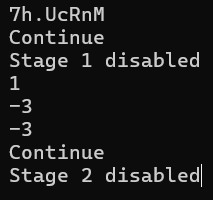
\includegraphics[width=0.2\textwidth]{s2-3.png}
\end{center}
\vspace{1ex}

\subsection{Tercera etapa}
El procedimiento \texttt{main} realiza una llamada a \texttt{Stage3} mediante la instrucción \texttt{call Stage3}. Procediendo de manera análoga a las etapas anteriores, accedemos al procedimiento utilizando \texttt{F11} y desensamblamos su contenido, obteniendo el siguiente resultado:

\begin{center}
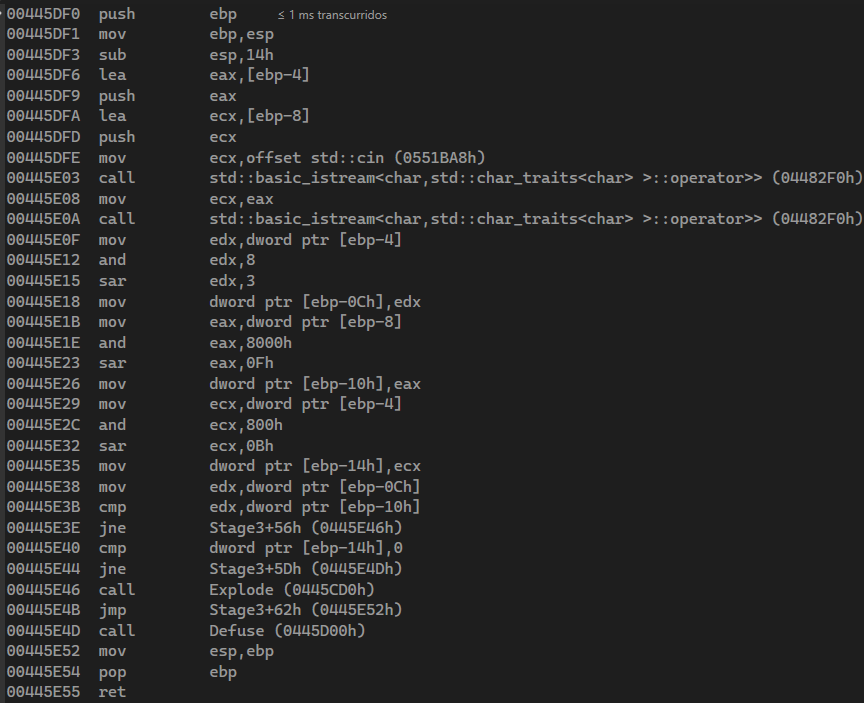
\includegraphics[width=0.9\textwidth]{s3-1.png}
\end{center}

\vspace{3ex}

\noindent En esta ocasión, el procedimiento consiste en la lectura de dos valores numéricos introducidos por el usuario, para posteriormente analizar y comparar ciertos bits específicos de estos números a fin de verificar condiciones precisas.\vspace{2ex}

\subsubsection{Condiciones para los valores introducidos}
\noindent El procedimiento \texttt{Stage3} se desarrolla de la siguiente manera:
\begin{enumerate}
  \item \textbf{Preparación inicial:} Se guarda el valor actual de \texttt{ebp} y se reserva espacio en la pila para variables locales:\vspace{1ex}
  \begin{lstlisting}[style=assemblyStyle]
    00445DF0  PUSH ebp
    00445DF1  MOV ebp, esp
    00445DF3  SUB esp, 14h
  \end{lstlisting}
  \vspace{1ex}

  \item \textbf{Lectura de números:} Se solicitan dos valores al usuario mediante \texttt{std::cin}:
  \begin{itemize}
    \item El primer número se almacena en \texttt{[ebp-8]}: \vspace{1ex}
    \begin{lstlisting}[style=assemblyStyle]
      00445DF6  LEA eax, [ebp-4]
      00445DF9  PUSH eax
      00445DFA  LEA ecx, [ebp-8]
      00445DFD  PUSH ecx
      00445DFE  MOV ecx, offset std::cin
      00445E03  CALL std::basic_istream<char>::operator>>
    \end{lstlisting}
    \vspace{1ex}

    \item El segundo número se almacena en \texttt{[ebp-4]}: \vspace{1ex}
    \begin{lstlisting}[style=assemblyStyle]
      00445E08  MOV ecx, eax
      00445E0A  CALL std::basic_istream<char>::operator>>
    \end{lstlisting}
  \end{itemize}
  \vspace{1ex}

  \item \textbf{Procesamiento:} Se realizan operaciones de enmascaramiento y desplazamiento de bits sobre los números ingresados:
  \begin{itemize}
    \item Al segundo número leído (\texttt{[ebp-4]}), se le aplica una máscara \texttt{0x8} (seleccionando el bit 3) y se desplaza tres posiciones a la derecha, almacenándose el resultado en \texttt{[ebp-0Ch]}: \vspace{1ex}
    \begin{lstlisting}[style=assemblyStyle]
      00445E0F  MOV edx, dword ptr [ebp-4]
      00445E12  AND edx, 8
      00445E15  SAR edx, 3
      00445E18  MOV dword ptr [ebp-0Ch], edx
    \end{lstlisting}
    \vspace{1ex}

    \item Al primer número leído (\texttt{[ebp-8]}), se le aplica una máscara \texttt{0x8000} para aislar el bit 15, desplazándolo posteriormente 15 posiciones hacia la derecha y almacenando el resultado en \texttt{[ebp-10h]}.

    \item Igualmente, al segundo número leído (\texttt{[ebp-4]}) se le aplica una máscara \texttt{0x800} (bit 11) y se desplaza once posiciones a la derecha, almacenándose en \texttt{[ebp-14h]}.
  \end{itemize}
  \vspace{1ex}

  \item \textbf{Comprobaciones:} Se realizan verificaciones específicas sobre los bits procesados:
  \begin{itemize}
    \item Si el valor almacenado en \texttt{[ebp-0Ch]} (bit 3 del segundo número) difiere del valor de \texttt{edx}, se activa la bomba: \vspace{1ex}
    \begin{lstlisting}[style=assemblyStyle]
      00445E38  CMP dword ptr [ebp-0Ch], edx
      00445E3B  JNE Stage3+56h (00445E4Eh)
    \end{lstlisting}
    \vspace{1ex}
    \item Si el bit 15 del primer número (\texttt{[ebp-10h]}) es igual a 1, el programa explota. \vspace{1ex}
    \item Si el bit 11 del segundo número (\texttt{[ebp-14h]}) es igual a 1, el programa igualmente explota. \vspace{1ex}
  \end{itemize}

  \item \textbf{Finalización:} Si todas las condiciones son satisfechas correctamente, el procedimiento invoca a \texttt{Defuse} y retorna al \texttt{main} utilizando la instrucción \texttt{ret}, de manera análoga a las fases anteriores.
\end{enumerate}
\vspace{1ex}

\noindent Tras la correcta introducción de los valores y la verificación exitosa de las condiciones, se invoca \texttt{Defuse} y, al regresar al procedimiento principal, se observará el siguiente estado en Visual Studio:

\begin{center}
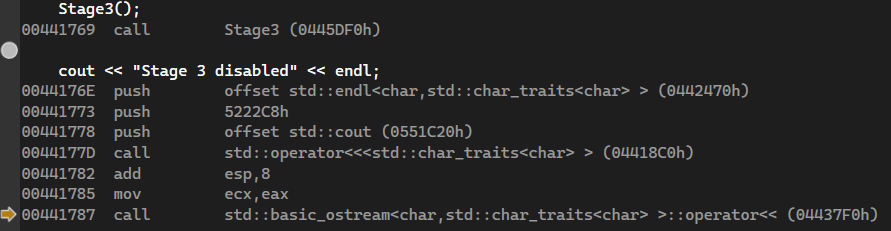
\includegraphics[width=0.95\textwidth]{s3-2.png}
\end{center}
\noindent Y la consola presentará el siguiente aspecto:
\begin{center}
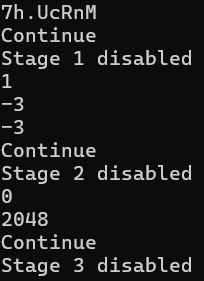
\includegraphics[width=0.3\textwidth]{s3-3.png}
\end{center}
\vspace{3ex}

\subsection{Cuarta etapa}

Finalmente, en el procedimiento \texttt{main}, se realiza una llamada a la cuarta etapa mediante \texttt{call Stage4}. Procediendo de manera análoga a los casos anteriores, accedemos al procedimiento utilizando \texttt{F11} y desensamblamos su contenido, obteniendo el siguiente resultado:

\begin{center}
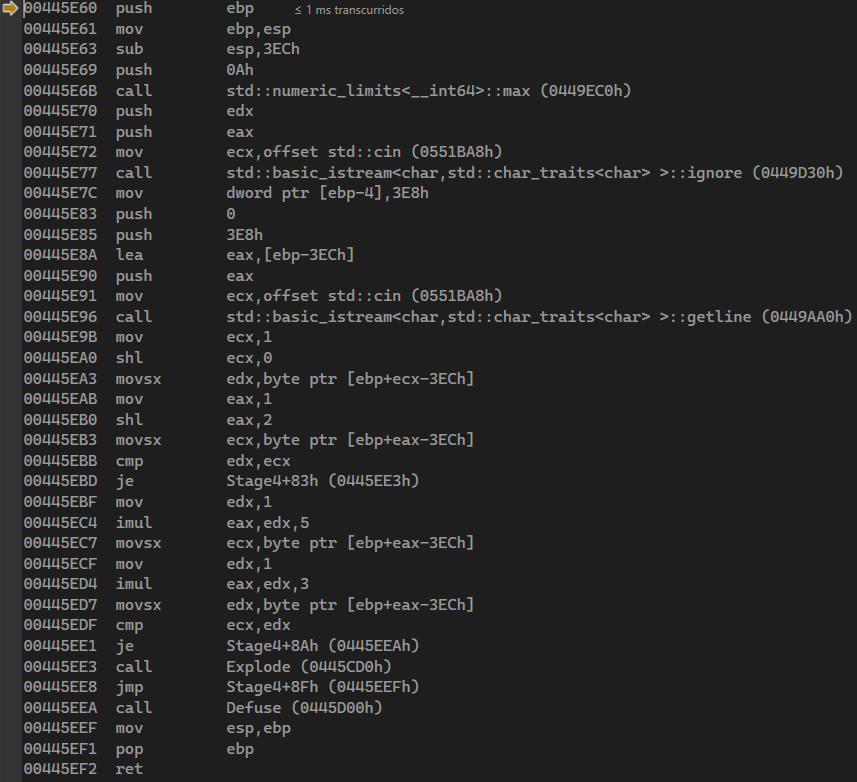
\includegraphics[width=0.95\textwidth]{s4-1.png}
\end{center}
\vspace{1ex}

\noindent En esta fase, el programa solicita al usuario la introducción de una línea completa de texto, para posteriormente realizar diversas comprobaciones entre caracteres específicos de la cadena.\vspace{2ex}

\subsubsection{Condiciones para la cadena introducida}
\noindent El procedimiento \texttt{Stage4} se desarrolla de la siguiente manera:
\begin{enumerate}
  \item \textbf{Preparación inicial:} Se guarda el registro \texttt{ebp} y se reserva espacio en la pila para el almacenamiento de datos:\vspace{1ex}
  \begin{lstlisting}[style=assemblyStyle]
    00445E60 PUSH ebp
    00445E61 MOV ebp, esp
    00445E63 SUB esp, 3ECh
  \end{lstlisting}
  \vspace{1ex}

  \item \textbf{Lectura de datos:} Se solicita al usuario una línea completa mediante la función \texttt{std::getline}: \vspace{1ex}
  \begin{lstlisting}[style=assemblyStyle]
    00445E7C MOV eax, [ebp-4]
    00445E83 PUSH 3E8h
    00445E88 LEA eax, [ebp-3ECh]
    00445E8B PUSH eax
    00445E8C MOV ecx, offset std::cin
    00445E91 CALL std::getline
  \end{lstlisting}
  \vspace{3ex}

  \item \textbf{Procesamiento de caracteres:} Se accede inicialmente al segundo carácter de la cadena: \vspace{1ex}
  \begin{lstlisting}[style=assemblyStyle]
    00445E98 MOV ecx, 1
    00445E9D SHL ecx, 0
    00445EA0 MOVSX edx, byte ptr [ebp+ecx-3ECh]
  \end{lstlisting}
  \vspace{1ex}
  De manera similar, se extrae el tercer carácter para su posterior comparación. \vspace{1ex}

  \item \textbf{Comprobación:} Se realizan dos comprobaciones principales:
  \begin{itemize}
    \item En primer lugar, si el segundo y el tercer carácter de la cadena son idénticos, se invoca inmediatamente al procedimiento \texttt{Explode}: \vspace{1ex}
    \begin{lstlisting}[style=assemblyStyle]
      00445EAE CMP ecx, edx
      00445EB0 JE Stage4+83h (00445EE3h)
    \end{lstlisting}
    \vspace{1ex}

    \item Si esta condición no se cumple, el programa continúa y compara el cuarto carácter con el sexto. Si estos dos caracteres son iguales, se invoca el procedimiento \texttt{Defuse}:\vspace{1ex}
    \begin{lstlisting}[style=assemblyStyle]
      00445EB2 MOV edx, 1
      00445EB7 IMUL eax, edx, 5
      00445EBC MOVSX ecx, byte ptr [ebp+eax-3ECh]
      00445EBF MOV edx, 1
      00445EC4 IMUL eax, edx, 3
      00445EC9 MOVSX edx, byte ptr [ebp+eax-3ECh]
      00445ECC CMP ecx, edx
    \end{lstlisting}
  \end{itemize}
  \vspace{1ex}

  \item \textbf{Finalización:} Si las condiciones de comprobación son correctas y la bomba no detona, el procedimiento se finaliza adecuadamente retornando al \texttt{main} mediante la instrucción \texttt{ret}, tal como sucedió en las etapas anteriores.
\end{enumerate}

\noindent Tras la correcta ejecución de esta cuarta etapa, el control retorna al procedimiento principal, observándose el siguiente estado en la consola:
\begin{center}
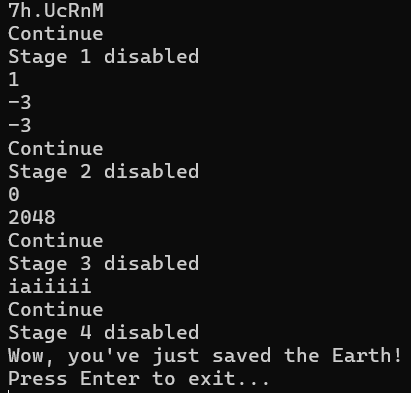
\includegraphics[width=0.3\textwidth]{s4-3.png}
\end{center}

\noindent Esto es debido a que se han desactivado exitosamente todas las etapas de la bomba y, por ello, se muestra el mensaje de \textit{``Wow, you've saved the Earth''}. Posteriormente, al presionar la tecla \texttt{Enter}, el programa se cierra retornando el valor 1 en el procedimiento \texttt{main}.\vspace{10ex}

\noindent Y en este caso, el código de Visual Studio presentará el siguiente aspecto:
\begin{center}
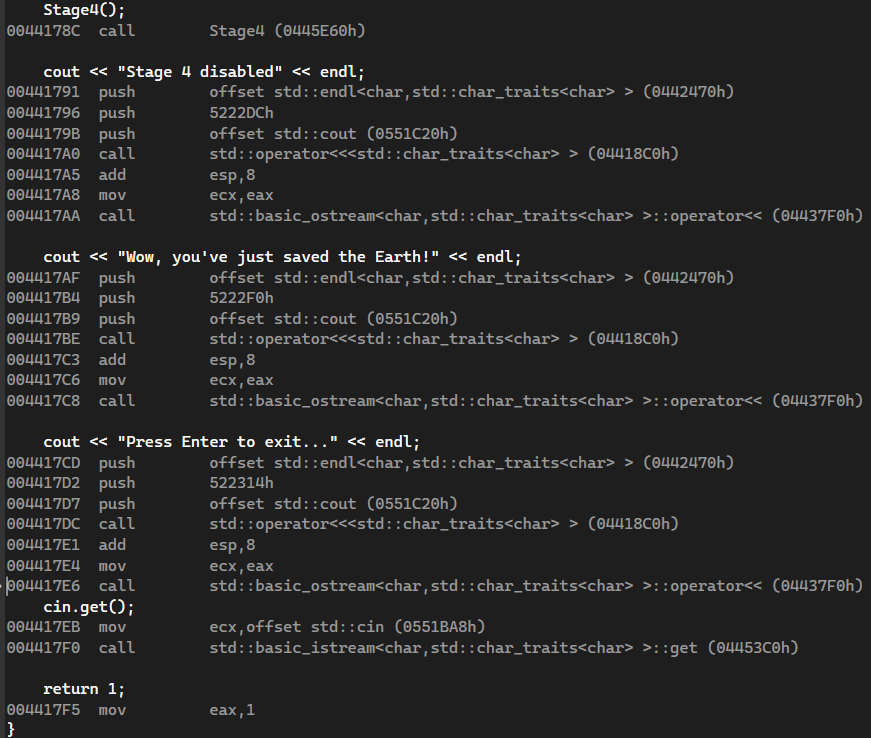
\includegraphics[width=0.95\textwidth]{s4-2.png}
\end{center}
\vspace{3ex}

\section{Como desactivar la bomba (y no morir en el intento)}
Como hemos visto previamente, para la correcta desactivación de la bomba, algunas posibles entradas válidas son:
\begin{enumerate}
  \item \texttt{7h.UcRnM} para la primera etapa.
  \item \texttt{1, -3, -3} para la segunda etapa.
  \item \texttt{0, 2048}
  \item \texttt{iaaaaa} para la cuarta etapa.
\end{enumerate}
\vspace{2ex}

\noindent De forma similar, se pueden plantear cadenas que romperían el programa, como por ejemplo:
\begin{enumerate}
  \item \texttt{UwU} para la primera etapa.
  \item \texttt{6, 6, 6} para la segunda etapa.
  \item \texttt{314159, 271828} para la tercera etapa.
  \item \texttt{hespaña} para la cuarta etapa.
\end{enumerate}
\vspace{3ex}

\section{Modificación del ejecutable}

El procedimiento llevado a cabo para modificar el ejecutable ha seguido una metodología similar a la aplicada durante las fases de análisis anteriores. Se ha empleado el desensamblador integrado en Visual Studio para examinar el código binario de la bomba, el cual, como se ha descrito previamente, está estructurado en cuatro etapas, invocadas mediante instrucciones \texttt{call}.\vspace{2ex}

\noindent Con el objetivo de evitar la ejecución de las distintas etapas sin alterar las entradas, se procedió a modificar las instrucciones de llamada (\texttt{call}) sustituyéndolas por instrucciones de no operación (\texttt{nop}), empleando para ello el editor hexadecimal \texttt{HxD}.\vspace{2ex}

\subsection{Primera llamada}
\noindent En el desensamblado, la llamada al procedimiento \texttt{Stage1} se observa de la siguiente forma:
\begin{center}
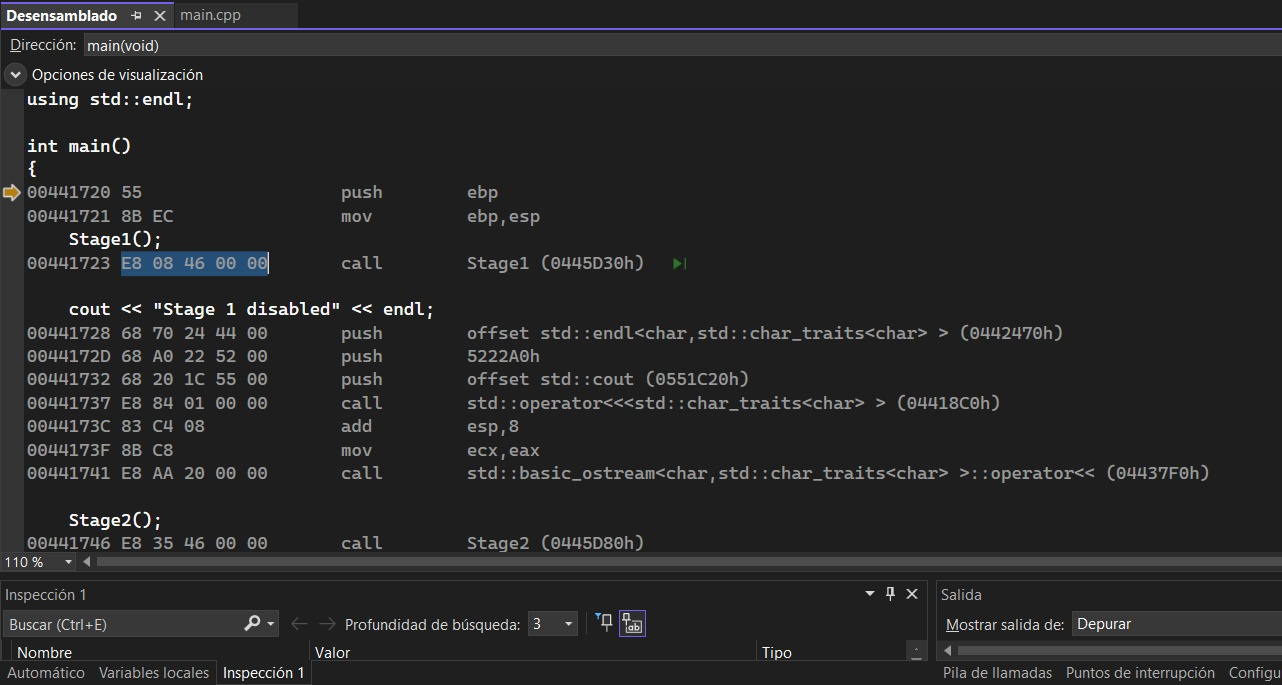
\includegraphics[width=0.95\textwidth]{4-1.png}
\end{center}
\vspace{2ex}

\noindent Posteriormente, utilizando la herramienta \texttt{HxD}, se localizó la secuencia de bytes \texttt{E8 82 46 00 00}, correspondiente a la instrucción de llamada al procedimiento \texttt{Stage1}:
\vspace{1ex}
\begin{center}
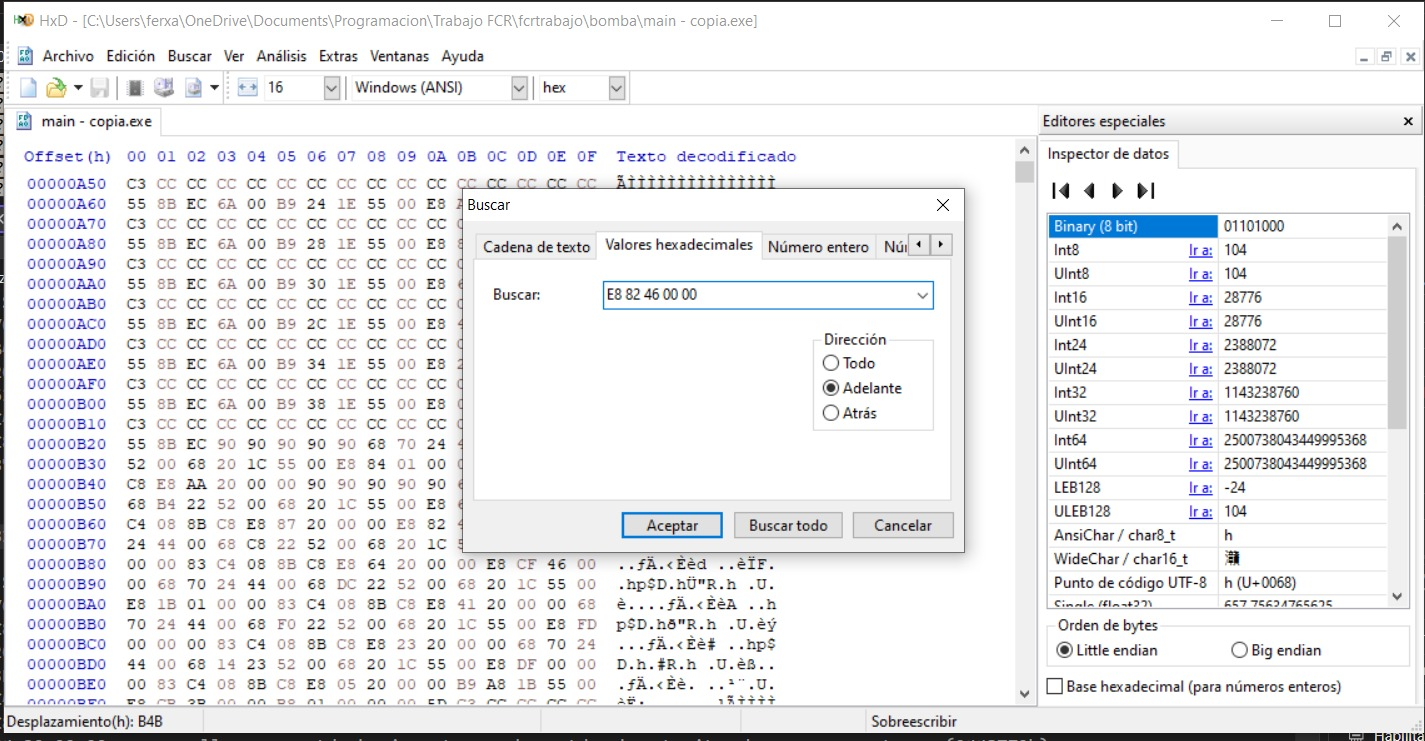
\includegraphics[width=0.95\textwidth]{4-4.png}
\end{center}
\vspace{2ex}

\noindent Esta secuencia fue reemplazada por:
\begin{center}
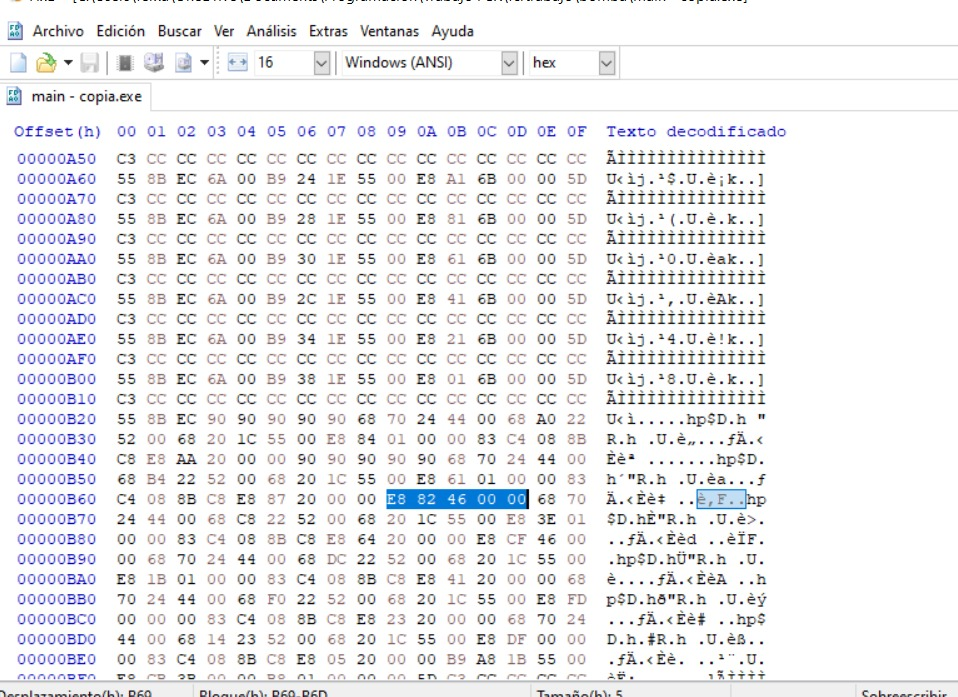
\includegraphics[width=0.57\textwidth]{4-5.png}
\end{center}
\vspace{1ex}

\noindent y posteriormente modificada a \texttt{90 90 90 90 90}, donde cada \texttt{90} corresponde a una instrucción \texttt{nop}:
\vspace{1ex}
\begin{center}
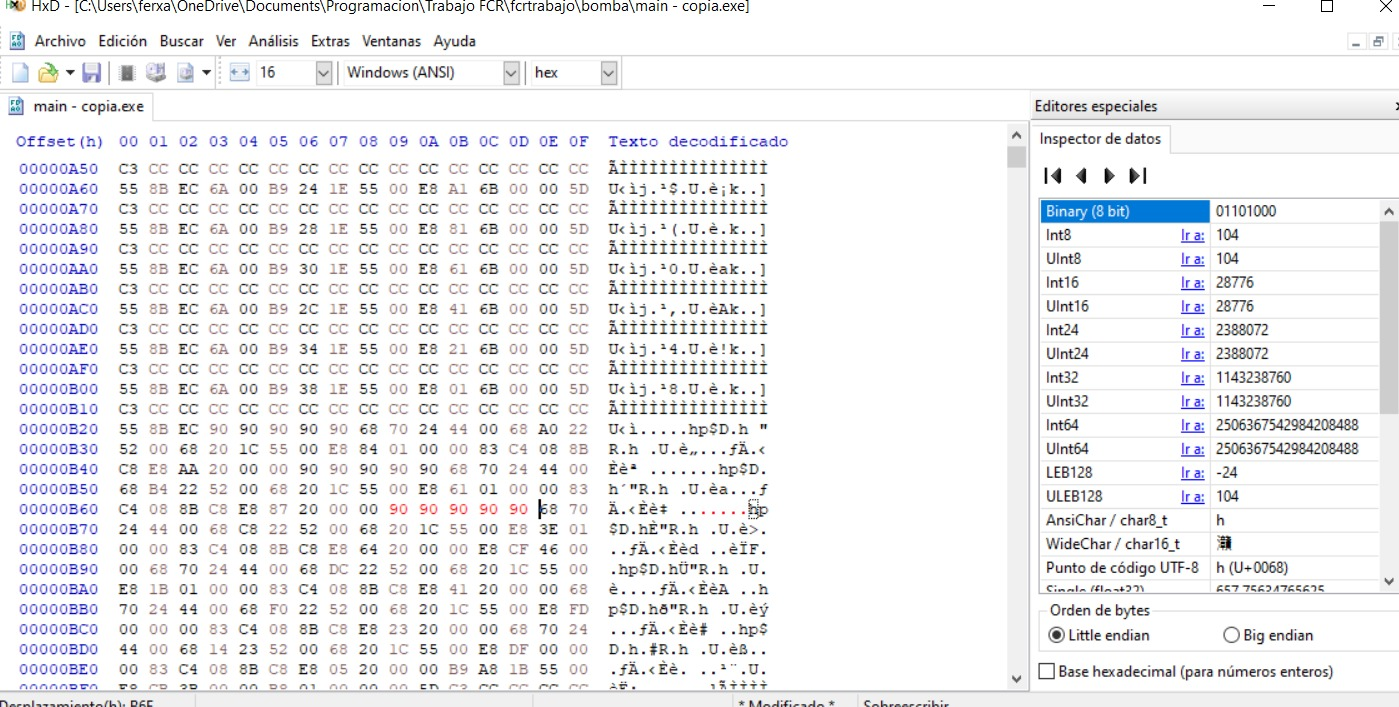
\includegraphics[width=0.7\textwidth]{4-6.png}
\end{center}
\vspace{2ex}

De este modo, al ejecutarse el programa, en lugar de realizar la llamada al procedimiento \texttt{Stage1}, simplemente se ejecutan instrucciones \texttt{nop}, que no alteran el flujo del programa, permitiendo así avanzar a la siguiente instrucción de forma segura.

\vspace{2ex}

\subsection{Segunda llamada}
\noindent Aplicando el mismo procedimiento, se localizó la llamada correspondiente a la segunda etapa, cuya secuencia de bytes es \texttt{E8 35 46 00 00}:
\begin{center}
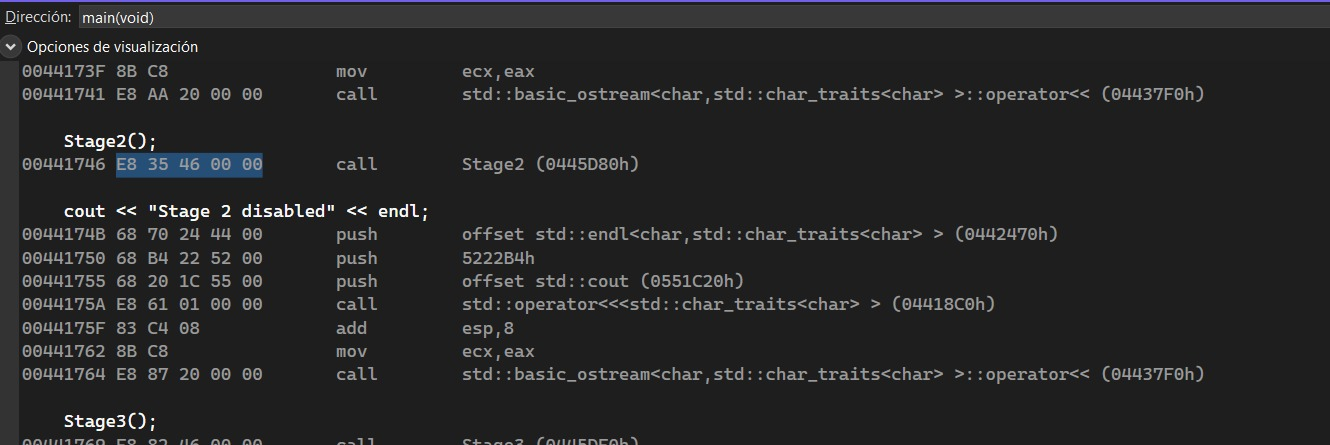
\includegraphics[width=0.85\textwidth]{4-2.png}
\end{center}

\noindent Esta instrucción también fue reemplazada por instrucciones \texttt{nop}, inhabilitando así la ejecución de \texttt{Stage2}.

\vspace{3ex}

\subsection{Tercera llamada}
\noindent Del mismo modo, para el procedimiento \texttt{Stage3}, la llamada identificada fue:
\begin{center}
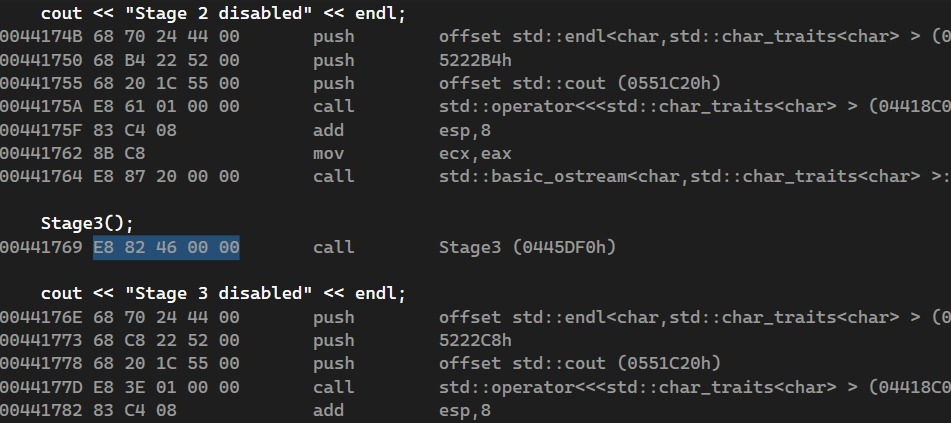
\includegraphics[width=0.85\textwidth]{4-3.png}
\end{center}
\vspace{1ex}

\noindent La cual se corresponde igualmente con la secuencia de bytes \texttt{E8 82 46 00 00}, que fue sustituida por instrucciones \texttt{nop} para anular la llamada.

\vspace{3ex}

\subsection{Cuarta llamada}
\noindent Finalmente, la llamada al procedimiento \texttt{Stage4} estaba representada por la secuencia de bytes \texttt{E8 CF 46 00 00}:
\begin{center}
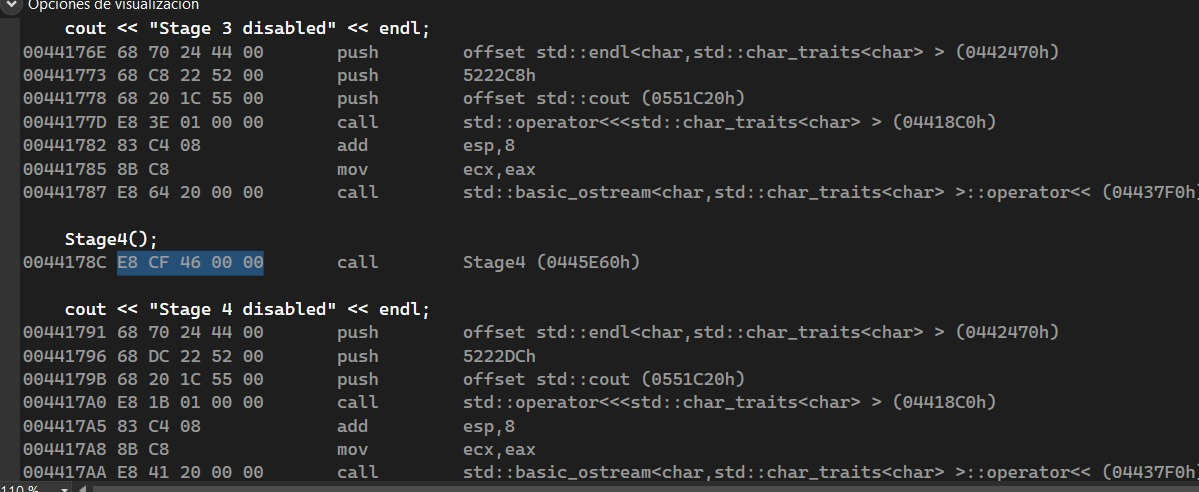
\includegraphics[width=0.9\textwidth]{4-7.png}
\end{center}
\vspace{1ex}

\noindent Esta última llamada fue igualmente modificada para evitar su ejecución mediante la sustitución por instrucciones \texttt{nop}.

\vspace{2ex}

\noindent De esta manera, al ejecutar el programa modificado, todas las llamadas a las etapas son omitidas, avanzando directamente en el flujo de \texttt{main}. Como resultado, el programa muestra inmediatamente el mensaje que indica la desactivación exitosa de la bomba:

\begin{center}
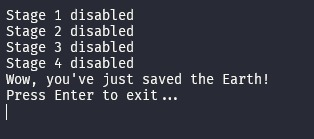
\includegraphics[width=0.3\textwidth]{4-8.png}
\end{center}
\vspace{3ex}



\section{Distribución del trabajo}
\subsection{Estrategia de trabajo}
La implementación del proyecto se ha organizado siguiendo una estrategia de trabajo colaborativo, basada en la asignación individual de cada una de las funciones principales descritas en el enunciado. Para el reparto del trabajo, en este caso fue algo más complejo que la última vez debido a que la división no era tan sencilla. \vspace{2ex}

\noindent Como soporte para el trabajo en equipo, se ha utilizado el sistema de control de versiones distribuido \textit{Git} en combinación con la plataforma \textit{Github} como repositorio remoto centralizado. En este caso particular, dado que no se requería de implementaciones de código simultáneas, no se ha requerido un flujo de trabajo basado en \textit{features branches}. En esta fase, otra herramienta empleada ha sido \textit{Discord},q ue es un servicio de mensajería instantánea y VoIP, que ha facilitado la comunicación entre los miembros del grupo. \vspace{2ex}

\noindent Gracias a estas herramientas, se ha podido llevar a cabo un trabajo colaborativo eficiente, permitiendo a cada miembro del grupo realizar sus aportaciones de manera individual y realizar una propuesta en común de los resultados obtenidos.

\noindent El repositorio que ha servido como entorno de trabajo colaborativo se encuentra alojado en la plataforma \textit{GitHub}, bajo el siguiente enlace: \href{https://github.com/PabloGarPe/fcrtrabajo}{https://github.com/PabloGarPe/fcrtrabajo}. A diferencia de la primera fase, para la entrega este repositorio ya se encontrará abierto públicamente.\vspace{5ex}

\subsection{Distribución de tareas}
Tal como se ha expuesto anteriormente, la distribución de tareas se ha estructurado en torno a la asignación individual de las partes del trabajo a los distintos integrantes del grupo. Tras el análisis individual se realizó una puesta en común de los resultados obtenidos, con el fin de que todos los miembros del grupo tuvieran un conocimiento general de la práctica y de los resultados obtenidos, además de facilitar la realización de la memoria. \vspace{2ex}

\noindent A continuación, se detalla la asignación específica de tareas realizada por cada miembro del equipo: \vspace{1ex}
\begin{center}
  \renewcommand{\arraystretch}{1.2}
  \begin{tabular}{|c|c|}
    \hline
    \textbf{Integrante}\cellcolor{azulSuave} & \textbf{Función implementada}\cellcolor{azulSuave} \\
    \hline
    Diego Díaz Mendaña & \textit{Stage 2} y \textit{memoria} \\
    Pablo García Pernas & \textit{Stage 1} y \textit{Stage 3} \\
    Fernando Suárez Fernández & \textit{Modificación del exe} \\
    Jorge Gota Ortín & \textit{Stage 4} \\
    \hline
  \end{tabular}
\end{center}
\vspace{3ex}

\subsection{Tiempos de desarrollo}
A continuación, se especifica el tiempo estimado invertido por cada miembro, considerando tanto las tareas individuales como las actividades colaborativas de revisión y coordinación: \vspace{2ex}
\begin{center}
  \renewcommand{\arraystretch}{1.2}
  \begin{tabular}{|c|c|}
    \hline
    \textbf{Integrante}\cellcolor{azulSuave} & \textbf{Tiempo dedicado}\cellcolor{azulSuave} \\
    \hline
    Diego Díaz Mendaña & 4 horas y 30 minutos \\
    Pablo García Pernas & 3 horas y 30 minutos \\
    Fernando Suárez Fernández & 3 horas, 33 minutos y 33 segundos \\
    Jorge Gota Ortín & 3 horas y 30 minutos\\
    \hline
  \end{tabular}
\end{center}

\end{document}